\section{Voltage Supplies}\label{sec:voltage-supplies}

	\subsection{Power Supplies}\label{ssec:power-supplies}
		In order to avoid any interference of the AC line, this project will work with a DC voltage input and any other necessary voltages will be acquainted from this higher input voltage supply.There are many different types of voltage regulators, nowadays the most common DC/DC being switching regulators. They are more efficient than linear regulators and consequently they waste less heat, the downside is the cost (due their consequently) and that they tend to have some ripple at the output \cite{schweber2017}. However, as the ripple can easily be filtered and that a switching power supply allows the input voltage to be of a much bigger range, this solution was considered the best for the project. 

		\subsubsection{5V Supply}\label{sssec:5v-supply}
			The voltage supply was choosen to be a 5V DC supply because all the components can work with this voltage. The choosen voltage regulator for the 5V supply was the TL2575-05 from \textit{Texas Instruments} \cite{tl2575-05-datasheet}, it has a output up to 1A, voltage drop of 2V, typical efficiency of 88$\%$ and can work with a 7 to 42V input. Figure \ref{fig:tl2575-05-circuit} shows the circuit used for the 5V supply.

			\begin{figure}[htbp]
				\centering
					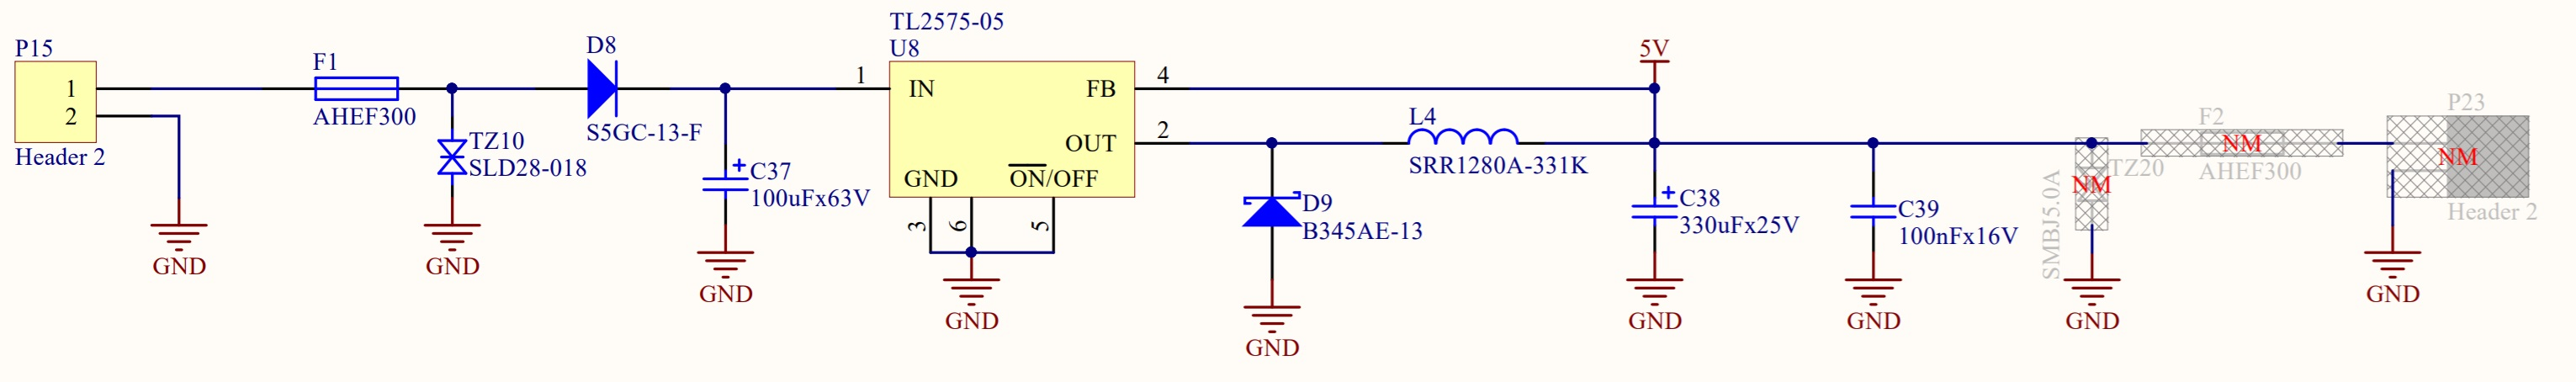
\includegraphics[width=.8\textwidth]{figuras/fig-tl2575-05-circuit.png}
				\caption{5V Power Supply Circuit}
				\label{fig:tl2575-05-circuit}
			\end{figure}

			According to \cite{tl2575-05-datasheet}, the main components to be choosed for the switching regulator are L4, C38 and D9. The inductor and the capacitor are used to form a LPF to transform the PWM output of the switching regulator to a DC voltage. D9 is a flyback diode used to shunt any negative current from the switching to ground and protect the device. The datasheet recommends using a 3A reverse current diode, a 330uH inductor and 330uF capacitor for the 5V regulator.

			The other components of the circuit are:

			\begin{itemize}
				\item\textit{TZ10 and TZ20}: TVS diodes to clamp to protect the input and output from ESD.
				\item\textit{F1 and F2}: resetable fuses, they will limit the current that flows into the circuit and protect the TVS.
				\item\textit{D8}: A diode to protect the input from inverse polarity.
				\item\textit{C37}: Input bypass capacitor recommended by the device's datasheet.
				\item\textit{C39}: Another bypass capacitor on the output to filter any residual noise.
			\end{itemize}

	\subsection{Voltage References}\label{ssec:voltage-references}

		In this project any power supply that the precision and stability of the output voltage is more concerning than the maximum output current will be called a voltage reference.

		\subsubsection{4V1 Reference}\label{sssec:4v1-reference}

			As said in Section \ref{ssec:thermocouple-sensor-detection}, the sensor detection circuit needs a 4V1 voltage reference for the comparator. This is achieved using the LM4040-4.1 from \textit{Microchip} \cite{lm4040-datasheet}. This is a fixed 4V1 precise voltage reference and according to the datsheet it has a tolerance of $\pm1.15\%$. Figure \ref{fig:4v1-voltage-ref} shows the circuit for the 4V1 voltage reference.

			\begin{figure}[htbp]
				\centering
					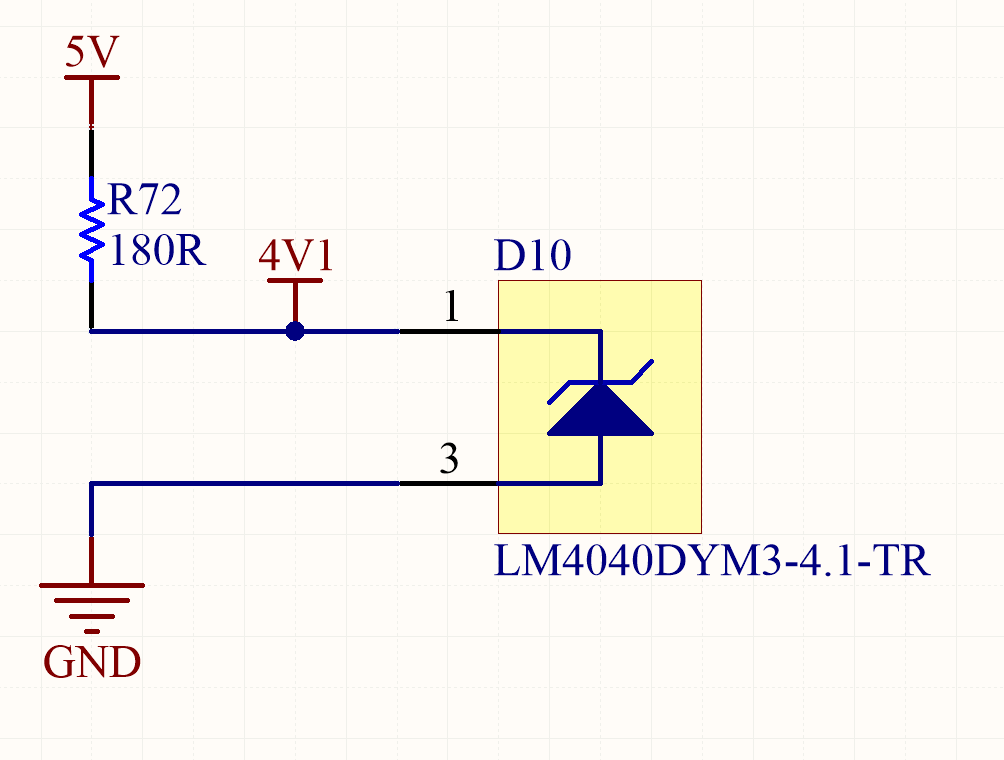
\includegraphics[width=.8\textwidth]{figuras/fig-4v1-voltage-ref}
				\caption{4V1 voltage reference circuit}
				\label{fig:4v1-voltage-ref}
			\end{figure}

			According to the datasheet the current flowing through the LM4040-4.1 must be never be greater than 15mA, voltage reference pins do need very little current, so a third of this 15mA will be taken as goal. Considering the voltage drop of 0.9V (5V - 4.1V) and the current of 5mA we need a 180$\Omega$ resistor in series with the regulator.